% set font and paper size
\documentclass[11pt,a4paper]{article}

% change to german
\usepackage[german]{babel}

% better hyphenation
\usepackage[final]{microtype}
\usepackage{csquotes}

% packages, images, math
\usepackage{geometry, graphicx, amsmath, amsfonts, array, multicol, multirow}

% bar charts
\usepackage{bchart}

% for bibliography
\usepackage[
    backend=biber,
    style=alphabetic,
    sorting=ynt,
    minalphanames=3,
]{biblatex}
\addbibresource{./res/references.bib}

% remove dots in ToC
\usepackage{tocloft}

% import line spacing
\usepackage{setspace}

% listings
\usepackage{listings}

% colors
\usepackage{xcolor}

% spacing between section titles and text
\usepackage{titlesec}
\titlespacing*{\section}{0pt}{0.7ex}{0.7ex}
\titlespacing*{\subsection}{0pt}{0.7ex}{0.7ex}
\titlespacing*{\subsubsection}{0pt}{0.7ex}{0.7ex}

% for urls
% break urls on line end
\usepackage[breaklinks, colorlinks=true, urlcolor=gray, citecolor=gray, linkcolor=black]{hyperref}

% Remove Indentation at new line
\setlength{\parindent}{0cm}

% Set Font to Arial, needs xelatex
\usepackage{unicode-math}
\usepackage{fontspec}
\setmainfont{Arial}

% Set Layout
\geometry{
    a4paper,
    left=25mm,
    right=25mm,
    top=25mm,
    bottom=20mm
}

% plots
\usepackage{pgfplotstable}
% recommended:
\usepackage{booktabs}
\usepackage{array}
\usepackage{colortbl}

\usepackage{pgfplots}

% moving in tikz picture
\usepackage{changepage}

% position figures
\usepackage{float}

% b tree
\usepackage{tikz}
\usetikzlibrary{shapes}

% set line spacing
\setstretch{1.5}

% remove ToC page number
\AtBeginDocument{\addtocontents{toc}{\protect\thispagestyle{empty}}} 

% bold caption
\usepackage[labelfont=bf]{caption}

% document
\begin{document}

% deckblatt
% title
\title{Schwierigkeiten bei Implementierung und Evaluation von Datenstrukturen in Datenbanksystemen}
\author{Anton Rodenwald (19)}
\maketitle

% page settings
\addtocounter{page}{-3}
\thispagestyle{empty}

\large
\begin{tabular}{l p{12cm}}

    Fachgebiet:          & Mathematik/Informatik      \\

    Wettbewerbssparte:   & Jugend Forscht             \\

    Bundesland:          & Niedersachsen              \\

    Wettbewerbsjahr:     & 2024                       \\

    Thema des Projektes: &
    In meinem Projekt wollte ich verschiedene in Datenbanksystemen genutzte Datenstrukturen
    implementieren und testen. Dabei betrachtete ich auch unterschiedliche Ansätze der
    Datenspeicherung und für den Datenzugriff. Bei den auftretenden Schwierigkeiten
    musste ich Lösungen finden bzw. etwas adaptieren. \\

    Projektbetreuerin:   & Birgit Ziegenmeyer         \\

    Institution:         & Schillerschule Hannover    \\
\end{tabular}

\clearpage

\pagestyle{empty}

% kurzfassung

\section*{Kurzfassung}

<Text>

\clearpage

% inhaltsverzeichnis

\renewcommand*\contentsname{Inhaltsverzeichnis}

\renewcommand{\cftdot}{}

\tableofcontents

\clearpage

\pagestyle{plain}

\section{Motivation, Fragestellung und Ziel}

Im Rahmen des Informatik Leistungkurses meiner Schule haben wir (Mitschüler und ich) uns
mit Datenbanken und Modellierung beschäftigt. Da jedoch auf die Funktionsweise einer
Datenbank nicht weiter eingegangen wurde und ich auch schon von Unterschiedlichen
Datenbankansätzen, genauer Relationalen und Nicht-Relationalen, gehört hatte,
wollte ich mich ihm Rahmen meines Projektes genauer damit beschäftigen.
Dazu wollte ich eine einfache Datenbank umsetzen.

\vspace*{0.3cm}

Meine Forschungsfrage ist deshalb, wie die Wahl der Datenstruktur die
Geschwindigkeit einer Datenbank beeinflusst und inwiefern sich eine Datenstruktur
für gewisse Daten besser oder schlechter eignet.

\vspace*{0.3cm}

Mein Ursprüngliches Ziel war dabei die Programmierung einer Datenbank
mit den Datenstrukturen R-Tree, B-Tree, Binary-Tree und Graphen.
Davon konnte ich leider aufgrund der hohen Komplexität (Stand jetzt) vieles nicht umsetzen.

\section{Hintergrund}

\subsection{Arten von Daten und passende Datenstrukturen}

Um mir einen Überblick über das Themengebiet zu verschaffen recherchierte ich zuerst im Internet.
Dabei fand ich viele Informationen über die Arten von Daten und Datenbanksystemen,
allerdings nichts konkretes über Performance Vergleiche dieser.
Verschiedene Datenarten sind dabei räumliche, zeitliche, als Objekte modellierbare und stark vernetzte Daten
\cite{no_sql_wikipedia} \cite{indian_overview}.

\vspace*{0.3cm}

Räumliche Daten sind z. B. Kartendaten (Google Maps, OpenStreetMap). Bestimmte Landmarken oder Objekte
(Bäume, Mulleimer) lassen sich beispielsweise als Punkte auf einer Fläche modellieren.
Es müssen dann effizient Fragen wie z. B. ``Wie viele Mülleimer gibt es in diesem Park?'' oder ``Was sind
die 3 am besten bewerteten Restaurants in der Innenstadt?'' beantwortet werden.
Eine dafür ausgelegte Datenstruktur ist der R-Tree.

\vspace*{0.3cm}

Zeitliche Daten können z. B. die von einem Sensor gemessene Temperaturen sein.
Wichtig wäre dann z. B., dass man einfach Statistiken wie Durchschnittswerte bilden
oder Anomalien erkennen könnte.

\vspace*{0.3cm}

Daten, die klassischerweise in relationellen Datenbanken gespeichert werden,
lassen sich durch viele, gleich aufgebaute Objekte modellieren lassen.
Beispielsweise speichert ein Unternehmen über Kunden immer die gleichen Daten
(Name, E-Mail, ...). Jeder Datensatz kann dann eindeutig z. B. über eine
ID identifiziert. Eine dafür geeignete Datenstruktur ist der B-Tree, eine
dem Binary-Tree ähnliche Datenstruktur.

\vspace*{0.3cm}

Wenn zwischen einzelnen Daten wie z. B. jedem Nutzer einer Social Media Plattform
allerdings viele Beziehungen bestehen (Follower, Likes), so eignet sich ein Graph
als Datenstruktur besser.

\subsection{Arten von Datenbanksystemen}

Moderne Datenbanksysteme ermöglichen meist, mit einem System verschiedene
Speicherungsformen zu nutzen. Trotzdem muss man sich bei einem Multi-modalen System
natürlich überlegen, welche Daten man nun in welcher Art von Datenstruktur speichern
will. Die Website \href{https://db-engines.com/en/ranking}{db-engines.com} stellt z. B.
eine Übersicht über die aktuell beliebtesten Datenbanksysteme und deren Modalitäten dar.

\section{Vorgehen}

\subsection{Schwierigkeiten bei der Implementierung}

Mein geplantes Vorgehen bestand darin, ein Datenbanksystem mit diesen
verschiedenen Datenstrukturen in C++ umzusetzen.
Während dem Entwicklungsprozess und der Implementierung zeigte sich allerdings die
zunehmende Komplexität, weswegen ich nur begrenzt die verschiedenen Datenstrukturen
vergleichen konnte. Trotzdem werde die angestrebten Datenstrukturen
zumindest in ihrer Funktion erläutern und meine Schwierigkeiten bei der Umsetzung
beschreiben, sodass sie anderen vielleicht nicht passieren.
Auch werde ich meine dann tatsächlich durchgeführten Tests beschreiben.
Also ein normaler Entwicklungsprozess ganz nach dem Zitat

\begin{quote}
    \guillemetright we do these things not because they are easy, \\
    but because we thought they were going to be easy \guillemetleft
\end{quote}

\subsubsection{Beej und <sys/socket.h>}
Zu Beginn meines Projektes folgte ich einem guten \href{https://beej.us/guide/bgnet/html/}{Tutorial}
von Brian Hall, um Kommunikation über Linux Websockets umzusetzen, da Datenbanksysteme
eine Schnittstelle zu anderen Programmen benötigen.
Da mein Datenbank-Backend allerdings nicht rechtzeitig ausgereift genug war, konnte
ich diese Schnittstelle noch nicht in Kombination mit dem Rest testen.

\subsubsection{Probleme bei B-Tree und Binary-Tree}

Da der B-Tree eine in vielen Datenbanken verwendete Datenstruktur ist, wollte ich
diesen zuerst implementieren. Als Grundlage nahm ich die erste Veröffentlichung über
diese durch 2 Boeing Entwickler \cite{boeing_engineers}.

\vspace*{0.3cm}

Der B-Tree ist dabei ähnlich zu einem Binären Suchbaum.
Der Hauptunterschied ist, das jeder Node nicht nur 2 Child Nodes
hat, wodurch der Baum weniger tief ist.
Um Elemente zu Suchen, zu Löschen oder zu Ändern folgt man der Baumstruktur vom
Root Node ausgehend. Durch Vergleiche innerhalb der Nodes und das traversieren der
Äste findet man ein bestimmtes Elemente oder eine Position im Baum.

\begin{center}
    \begin{tikzpicture}
        \tikzstyle{bplus}=[rectangle split, rectangle split horizontal,rectangle split ignore empty parts,draw]
        \tikzstyle{every node}=[bplus]
        \tikzstyle{level 1}=[sibling distance=80mm]
        \tikzstyle{level 2}=[sibling distance=15mm]
        \node {15} [->]
        child {node {3 \nodepart{two} 7}
                child {node {1 \nodepart{two} 2}}
                child {node {4 \nodepart{two} 6}}
                child {node {8 \nodepart{two} 9}}
            }
        child {node {21 \nodepart{two} 28 \nodepart{three} 32 \nodepart{four} 50}
                child[sibling distance=20mm] {node {17 \nodepart{two} 20}}
                child[sibling distance=20mm] {node {22 \nodepart{two} 25}}
                child[sibling distance=20mm] {node {28 \nodepart{two} 30}}
                child[sibling distance=25mm] {node {34 \nodepart{two} 38 \nodepart{three} 44 \nodepart{four} 47}}
                child[sibling distance=30mm] {node {53 \nodepart{two} 54 \nodepart{three} 60 \nodepart{four} 88}}
            }
        ;\end{tikzpicture}
\end{center}

Bei der Implementation des B-Tree traten allerdings einige Probleme auf.
Der Hauptgrund, warum ich mich dafür entschied, andere Datenstrukturen
zu testen war, dass die Ausbalancierung beim B-Tree relativ komplex ist.
Auch entschied ich mich, meine Tests ausschließlich mit im RAM liegenden Daten
durchzuführen, da eine Speicherung auf einer Festplatte noch mehr Komplexität bedeutet
hätte.

\vspace*{0.5cm}

Anschließend implementierte ich als Alternative dann einen AVL-Tree, eine sich selbst
ausbalancierende Variante des Binären Suchbaums (BST). Beim anschließenden
konzeptionieren der Performance-Tests entdeckte ich allerdings noch einen
beim einfügen von Elementen auftretenden Fehler, weswegen ich mich entschied,
auch diesen nicht zu testen.

\clearpage

\subsection{Testdaten und Test-Datenstrukturen}

\subsubsection{Testdaten}

Bei den Testdaten handelt es sich um eine fiktive Schülerschaft, in der jeder
Schüler Freundschaften und Feindschaften hat. Diese Testdaten generierte ich mir
mit einem Python Script und speicherte diese in einer CSV-Datei.
Jeder Schüler hat dabei eine ID und einen Namen, der eine zufällige Zeichenkette ist.
Anschließend sind bei jedem Schüler noch 100 Freund- und Feindschaften eingetragen.

\begin{lstlisting}
0, eszycidpyopumzgd, 255777-14862-..., 204372-226894-...
1, idixqgtnahamebxf, 233658-369416-..., 265451-355559-...
2, digztyrwpvlifrgj, 104446-129174-..., 188986-42660-...
...
\end{lstlisting}

\subsubsection{Testanforderungen}

Bei meinen Performance Tests verglich ich die Suchgeschwindigkeit der Datenstrukturen.
Die gleichen Testdaten wurden in beide Datenstrukturen eingelesen und anschließend
wurde gemessen, wie schnell auf einen bestimmten Teil der Daten jeweils zugegriffen
werden konnte. Einmal sollten alle Freunde von Schüler Nr. 2 und einmal alle
Feinschaften von Schüler Nr. 1 gefunden werden.

\subsubsection{Such-Array}

Auch aufgrund der vorigen Schwierigkeiten testete ich nun nicht
mit einem B-Tree oder Binary-Tree, sondern wendete die Binäre Suche
auf ein sortiertes Array an. Prinzipiell nutzen aber alle 3 Datenstrukturen die
Binäre Suche. Die Testdaten sind in diesem Fall auf 3 Such-Arrays (vgl. Tabellen)
aufgeteilt, jeweils eine für Schüler, Freundschaften und Feindschaften.

\begin{table}[H]
    \centering
    \begin{tabular}{|l|l|}
        \hline
        Schüler\_1\_ID & Schüler\_2\_ID \\ \hline
        5          & 7          \\ \hline
        5        & 75         \\ \hline
        5        & 456        \\ \hline
        5       & 45         \\ \hline
    \end{tabular}
    \qquad
    \begin{tabular}{|l|l|}
        \hline
        Schüler\_1\_ID & Schüler\_2\_ID \\ \hline
        7          & 629          \\ \hline
        7        & 762         \\ \hline
        7        & 229        \\ \hline
        7       & 29435         \\ \hline
    \end{tabular}
    \caption{Tabellenausschnitte Freundschaften/Feindschaften}
\end{table}

Um alle Freunde/Feinde eines Schülers zu finden, müssen in
den als Assoziationstabellen fungierenden, sortierten Such-Arrays
alle Datensätze zwischen dem kleinstmöglichen und größtmöglichen Wert
gefunden Werten. Beispielsweise für den Schüler $5$ alles zwischen den Datensätzen
$5 | 0$ und $5 | m$ wenn $m$ die Anzahl an Schülern ist. Da das Such-Array
nach beiden Spalten sortiert ist, muss nur mit der Binären Suche das linke
und rechte Ende des Bereichs bestimmt werden. Anschließend können in linearer
Zeit alle gesuchten Datensätze ausgelesen werden.

\vspace*{0.5cm}

\begin{figure}[H]
    \centering
    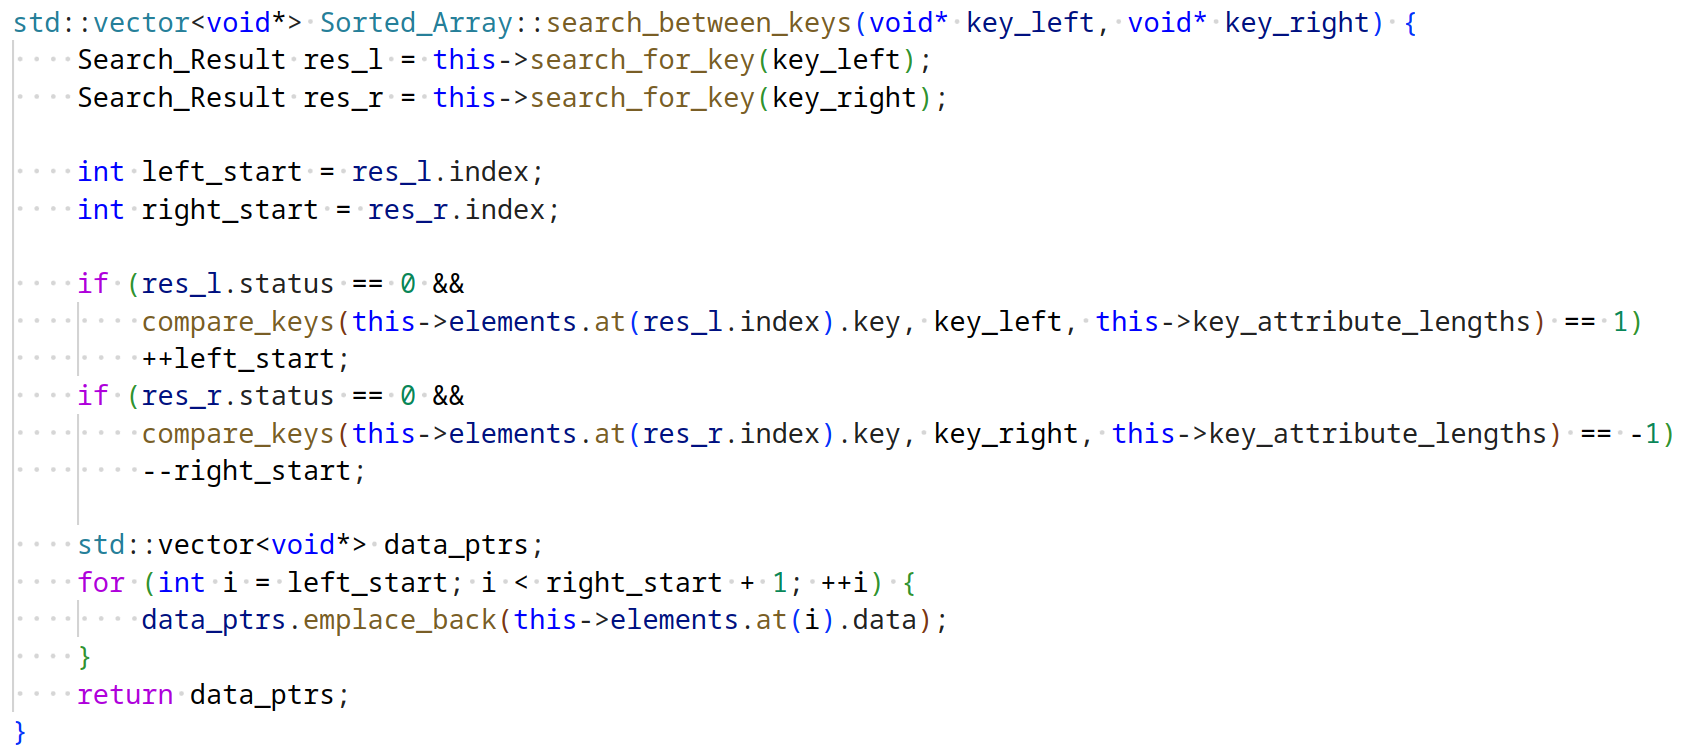
\includegraphics[width=1.1\textwidth]{./res/code_sort_array.png}
    \caption{C++ Code der Such-Array-Suchfunktion}
\end{figure}

\subsubsection{Graph}

Bei meiner Implementierung einer Graph-Datenstruktur sind in jedem Node
die Daten und die Verbindungen zu anderen Nodes gespeichert.
Um alle Freundschaften oder Feindschaften zu erhalten muss nur über diese
Daten iteriert werden und man erhält schnell die Daten der befreundeten oder
befeindeten Schüler. Die Art der Verbindung (Freund/Feind) kann dabei durch
das $link\_schema$ festgelegt werden.

\vspace*{0.5cm}

\begin{figure}[H]
    \centering
    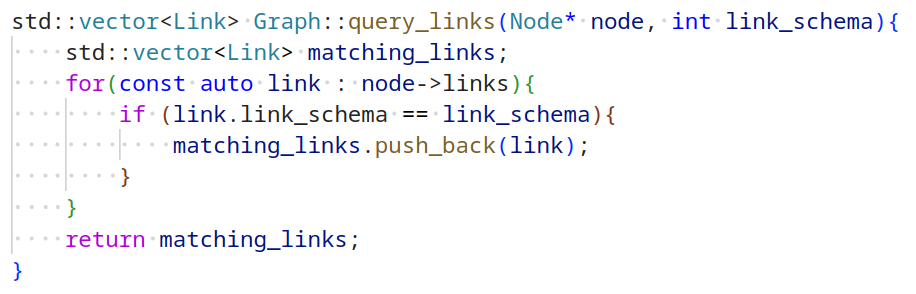
\includegraphics[width=1.0\textwidth]{./res/code_graphdb.png}
    \caption{C++ Code der Graph-Suchfunktion}
\end{figure}

\subsection{Komplexitäts Analyse}



\section{Messwerte}

Meine Messungen führte ich auf meinem Desktop PC und meinem Laptop (Plugged-In) durch.
Auf jedem Computer nahm ich 2 Messreihen auf.
Jede der 4 Anfragen and die 2 Datenstrukturen wurde jeweils 50-mal direkt hintereinander
ausgeführt.
$SA$ beschreibt die Datenstruktur Such-Array. $G$ stetht für Graph.
Das $F$ beschreibt die Suche nach allen Freunden des Schülers Nr. 2.
Das $H$ beschreibt die Suche nach allen Feindschaften (Hostilities) des Schülers Nr. 1.

\clearpage

\begin{figure}[H]
    \centering
    \begin{tikzpicture}[scale=1]
        \begin{axis}[
                x label style={at={(axis description cs:0.5,-0.01)},anchor=north},
                y label style={at={(axis description cs:-0.01,0.5)},anchor=south},
                xlabel=\textbf{Nummer der Messung},
                ylabel=\textbf{Zeit in Nanosekunden},
                width=1.0\textwidth,
                height=0.7\textwidth,
            ]
            \addplot table [y=$SA_F$, x=NR]{./res/data_pc_1.dat};
            \addlegendentry{$SA_F$ series}
            \addplot table [y=$SA_H$, x=NR]{./res/data_pc_1.dat};
            \addlegendentry{$SA_H$ series}
            \addplot table [y=$G_F$, x=NR]{./res/data_pc_1.dat};
            \addlegendentry{$G_F$ series}
            \addplot table [y=$G_H$, x=NR]{./res/data_pc_1.dat};
            \addlegendentry{$G_H$ series}
        \end{axis}
    \end{tikzpicture}
    \vspace*{-0.8cm}
    \caption{\textbf{1. Messreihe am PC (Ryzen 7 2700)}}
\end{figure}

\begin{figure}[H]
    \centering
    \begin{tikzpicture}[scale=1]
        \begin{axis}[
                x label style={at={(axis description cs:0.5,-0.01)},anchor=north},
                y label style={at={(axis description cs:-0.01,0.5)},anchor=south},
                xlabel=\textbf{Nummer der Messung},
                ylabel=\textbf{Zeit in Nanosekunden},
                width=1.0\textwidth,
                height=0.7\textwidth,
            ]
            \addplot table [y=$SA_F$, x=NR]{./res/data_pc_2.dat};
            \addlegendentry{$SA_F$ series}
            \addplot table [y=$SA_H$, x=NR]{./res/data_pc_2.dat};
            \addlegendentry{$SA_H$ series}
            \addplot table [y=$G_F$, x=NR]{./res/data_pc_2.dat};
            \addlegendentry{$G_F$ series}
            \addplot table [y=$G_H$, x=NR]{./res/data_pc_2.dat};
            \addlegendentry{$G_H$ series}
        \end{axis}
    \end{tikzpicture}
    \vspace*{-0.8cm}
    \caption{\textbf{2. Messreihe am PC (Ryzen 7 2700)}}
\end{figure}

\clearpage

\begin{figure}[H]
    \centering
    \begin{tikzpicture}[scale=1]
        \begin{axis}[
                x label style={at={(axis description cs:0.5,-0.01)},anchor=north},
                y label style={at={(axis description cs:-0.01,0.5)},anchor=south},
                xlabel=\textbf{Nummer der Messung},
                ylabel=\textbf{Zeit in Nanosekunden},
                scaled ticks=false,
                width=1.0\textwidth,
                height=0.7\textwidth,
            ]
            \addplot table [y=$SA_F$, x=NR]{./res/data_laptop_1.dat};
            \addlegendentry{$SA_F$ series}
            \addplot table [y=$SA_H$, x=NR]{./res/data_laptop_1.dat};
            \addlegendentry{$SA_H$ series}
            \addplot table [y=$G_F$, x=NR]{./res/data_laptop_1.dat};
            \addlegendentry{$G_F$ series}
            \addplot table [y=$G_H$, x=NR]{./res/data_laptop_1.dat};
            \addlegendentry{$G_H$ series}
        \end{axis}
    \end{tikzpicture}
    \vspace*{-0.8cm}
    \caption{\textbf{1. Messreihe am Laptop (Ryzen 5 5500U)}}
\end{figure}

\begin{figure}[H]
    \centering
    \begin{tikzpicture}[scale=1]
        \begin{axis}[
                x label style={at={(axis description cs:0.5,-0.01)},anchor=north},
                y label style={at={(axis description cs:-0.01,0.5)},anchor=south},
                xlabel=\textbf{Nummer der Messung},
                ylabel=\textbf{Zeit in Nanosekunden},
                scaled ticks=false,
                width=1.0\textwidth,
                height=0.7\textwidth,
            ]
            \addplot table [y=$SA_F$, x=NR]{./res/data_laptop_2.dat};
            \addlegendentry{$SA_F$ series}
            \addplot table [y=$SA_H$, x=NR]{./res/data_laptop_2.dat};
            \addlegendentry{$SA_H$ series}
            \addplot table [y=$G_F$, x=NR]{./res/data_laptop_2.dat};
            \addlegendentry{$G_F$ series}
            \addplot table [y=$G_H$, x=NR]{./res/data_laptop_2.dat};
            \addlegendentry{$G_H$ series}
        \end{axis}
    \end{tikzpicture}
    \vspace*{-0.8cm}
    \caption{\textbf{2. Messreihe am Laptop (Ryzen 5 5500U)}}
\end{figure}

\clearpage

\section{Deutung der Messwerte}

Bei den Messwerten am PC lässt sich erkennen, dass in den ersten paar Messungen die
benötigte Zeit deutlich höher ist als bei den restlichen, nachfolgenden Messungen.
Die benötigte Zeit aller Tests pendelt sich auf einem niedrigeren Niveau ein.
Gleiches ist auch am Laptop zu beobachten, wo die Messpunkte jedoch unregelmäßiger sind.
Dies lässt sich vermutlich auf eine Speicherung von Werten im CPU-Cache zurückführen,
in dem nach den ersten Durchläufen Daten vorgehalten werden, was zu besseren
Messergebnissen führt.
Vereinzelt gibt es auch in diesen Bereichen bei PC und Laptop ausreißende Werte.
Diese sind wahrscheinlich Messanomalien, erzeugt durch einmahlige Lastspitzen verursacht
durch andere Prozesse auf dem Testsystem oder durch Hardwarebedingte Faktoren.
Betrachtet man die 1. Messung, wo die Werte noch auseinanderliegen,
so lässt sich nicht feststellen, dass eine der Datenstrukturen schneller
ist als die anderen. Interessant ist bei diesen ersten Messwerten, dass die Messungen
auf gleich strukturierte Daten (Freundschaften und Feindschaften) deutlich voneinander
Abweichen. Nicht überraschend sind die abweichenden Niveaus von PC und Laptop,
da bei CPUs mit unterschiedlichem Leistungsniveau logischerweise auch andere
Performance-Werte erzeugt werden.

\section{Beantwortung der Forschungsfrage}

Abschließend lässt sich die Forschungsfrage insofern beantworten, als dass
die Wahl der Datenstruktur in diesem Fall keinen Einfluss auf die Zugriffsgeschwindigkeit
hat. Keine der Datenstrukturen scheint der anderen Überlegen.

\section{Schwierigkeiten und Limitationen}

implementation
nur ram
AMDuProf hat nicht funktioniert, weil keine ahnung
% https://community.amd.com/t5/server-gurus-discussions/amduprof-not-attaching-to-processes-on-linux/m-p/578286#M1589

\section{fazit}

gelernt
gdb
C/C++ experience mit gdb
b tree
socket api linux

\section{ausblick interessen geweckt}

% Quellen
% bjnet
% 

\begin{bchart}[min=0, max=30, scale=1.9]
    \bcbar[label=1, text=List Comprehension Python mit Konvertierung zu numba.typed list]{26.849}
    \smallskip
    \bcbar[label=2, text=\hspace{7cm}List Comprehension Python]{9.307}
    \smallskip
    \bcbar[label=3, text=\hspace{2cm}List Comprehension Python mit Numba]{1.148}
    \smallskip
    \bcbar[label=4, text=\hspace{2cm}NumPy np.random.randint mit Numba]{0.401}
    \smallskip
    \bcbar[label=5, text=\hspace{2cm}NumPy np.random.randint]{0.051}
    \smallskip
    \bcxlabel{\bf{Ausführungszeit in Sekunden}}
\end{bchart}

\clearpage

\cite{boeing_engineers}
\cite{indian_overview}
\cite{sql_ideas}
\cite{avl_tree_wikipedia}

% break urls
\emergencystretch=0.5em

\section{Quellenangaben}

\url{https://beej.us/guide/bgnet/html/}

\printbibliography[title={Literaturverzeichnis}]

\end{document}
